% ============================================================
%  chapter08_optimality_of_universal_agents_slides.tex
%  Chapter 8: Optimality of Universal Agents
%  An Introduction to Universal Artificial Intelligence
%  Hutter, Quarel & Catt --- CRC Press, 2024
% ============================================================
\documentclass[aspectratio=169,10pt]{beamer}

\usetheme{Madrid}
\usecolortheme{seahorse}
\usefonttheme{professionalfonts}

% -- packages ------------------------------------------------------------------
\usepackage{amsmath,amssymb,bm}
\usepackage{graphicx}
\usepackage{booktabs}
\usepackage{listings}
\usepackage{xcolor}
\usepackage{tikz}
\usetikzlibrary{shapes,arrows,positioning,calc}
\usepackage{mathtools}
\usepackage{array}
\usepackage{multirow}
\usepackage{makecell}
\usepackage{stmaryrd}

\graphicspath{{figures/}}

% -- listings style --------------------------------------------------------
\lstdefinestyle{pythonstyle}{
  language=Python,
  basicstyle=\ttfamily\scriptsize,
  keywordstyle=\color{blue}\bfseries,
  stringstyle=\color{orange},
  commentstyle=\color{green!50!black}\itshape,
  numberstyle=\tiny\color{gray},
  numbers=left,
  stepnumber=1,
  numbersep=5pt,
  frame=single,
  backgroundcolor=\color{gray!7},
  breaklines=true,
  showstringspaces=false,
  tabsize=2,
  captionpos=b,
}
\lstset{style=pythonstyle}

% -- beamer setup -----------------------------------------------------------
\setbeamertemplate{footline}[frame number]
\setbeamertemplate{navigation symbols}{}
\setbeamersize{text margin left=0.5cm, text margin right=0.5cm}

% -- convenient macros -------------------------------------------------------
\newcommand{\Bstr}{\mathbb{B}^*}
\newcommand{\explain}[1]{\par\smallskip{\footnotesize\itshape #1}\par}
\newcommand{\Msol}{\mathcal{M}_{sol}}
\newcommand{\Mcomp}{\mathcal{M}_{comp}}

% -- title -------------------------------------------------------------------
\title[UAI -- Ch.8 Optimality of Universal Agents]{An Introduction to Universal Artificial Intelligence}
\subtitle{Chapter 8: Optimality of Universal Agents}
\author{Based on Hutter, Quarel \& Catt}
\institute{CRC Press, 2024}
\date{}

% =============================================================================
\begin{document}
% =============================================================================

\begin{frame}
  \titlepage
  \begin{center}
  \small\itshape ``Perfection is achieved, not when there is nothing more to add,\\
  but when there is nothing left to take away.'' --- Antoine de Saint-Exup\'ery
  \end{center}
\end{frame}

\begin{frame}{Outline}
  \tableofcontents
\end{frame}

% =============================================================================
\section{8.1 Definitions of Optimality}
% =============================================================================

\begin{frame}[allowframebreaks]{Why We Need Many Notions of Optimality}
  To construct an optimal agent, we first have to say precisely what
  \textbf{optimal} means. This chapter surveys the many definitions of
  optimality that have been proposed for sequential decision-making agents,
  compares their relative strengths and weaknesses, and asks whether AIXI (or
  any other agent) can actually attain them.

  \bigskip
  \textbf{Roadmap of the chapter.}
  \begin{itemize}
    \item \textbf{Section 8.1} defines each optimality criterion in turn, and
      explains why it is useful and what problems it may have.
    \item \textbf{Section 8.2} shows how a Bayesian agent's behaviour can be
      made undesirable by a bad choice of prior, and argues why such priors
      will rarely be used in practice.
    \item \textbf{Section 8.3} explores fundamental obstacles that some of
      these optimality criteria run into, and under what circumstances
      optimal policies actually exist.
  \end{itemize}

  \bigskip
  \textbf{A quick preview of the five notions we will meet.}
  \begin{itemize}
    \item $\nu$ (nu)-\textbf{optimality}: maximal value in one known,
      fixed environment $\nu$ (nu) -- the ideal, but unrealistic for General
      AI since the true environment is never known in advance.
    \item \textbf{Asymptotic optimality}: the agent's value only has to
      approach the optimal value \emph{eventually}, as time $t\to\infty$.
      Comes in \emph{strong} (almost sure), \emph{in mean}, \emph{in
      probability}, and \emph{weak} (Ces\`aro average) flavours, from
      strongest to weakest.
    \item \textbf{Bayes-optimality}: maximal expected value under a
      Bayesian mixture over a whole class of environments -- arguably the
      most reasonable criterion, but not automatically asymptotically
      optimal.
    \item \textbf{Regret minimization}: comparing lifetime performance to an
      agent that already knows the true environment; a much stronger,
      finite-time notion than asymptotic optimality.
    \item \textbf{Pareto optimality}: no other agent does at least as well in
      every environment and strictly better in at least one. Very weak on
      its own, but its \emph{balanced} refinement coincides with
      Bayes-optimality.
  \end{itemize}
\end{frame}

% -----------------------------------------------------------------------------
\subsection{8.1.1 $\nu$-Optimality}
% -----------------------------------------------------------------------------

\begin{frame}[allowframebreaks]{8.1.1 Environment-Based ($\nu$-)Optimality}
  \textbf{Environment-based optimality}, or \emph{$\nu$ (nu)-optimality} for
  some environment $\nu$, states that a policy is optimal if it achieves the
  maximum possible value for every history. Recall (Chapter 6) that the
  value $V_\nu^\pi(h)$ of a policy $\pi$ in environment $\nu$ is the total
  expected (discounted) future reward, starting from history $h$.

  \begin{block}{Definition 8.1.1 (Optimal policy)}
    A policy $\pi$ is \emph{optimal} in an environment $\nu$ ($\nu$-optimal)
    iff for all histories, $\pi$ attains the optimal value:
    $$V_\nu^\pi(h) = V_\nu^*(h) \quad \text{for all } h \in (\mathcal{A}\times\mathcal{E})^*.$$
    The action $a$ is an \emph{optimal action} iff $a \in \arg\max_{a'}
    \pi_\nu^*(a'|h)$ for some $\nu$-optimal policy $\pi_\nu^*$.
  \end{block}
  \explain{$\pi$ is the agent's \textbf{policy} (its strategy for choosing
    actions given the history so far); $\nu$ is the true \textbf{environment}
    it faces; $V_\nu^\pi(h)$ is the value (expected future reward) that
    $\pi$ achieves in $\nu$ starting from history $h$; $V_\nu^*(h)$ is the
    best value \emph{any} policy could achieve there; $h=(a_1e_1,\dots)$ is a
    history of past action/percept pairs; $\mathcal{A}$ and $\mathcal{E}$
    are the action and percept spaces. A policy is $\nu$-optimal if it
    always matches the best possible value.}

  \bigskip
  If we knew the true environment $\nu$ in advance, we could choose $\nu=\mu$
  and build the agent $\mathrm{AI}\mu$ with policy $\pi_\nu^*$, which
  maximizes expected reward over its lifetime -- a very natural (if
  unrealistic) notion of optimality.
\end{frame}

\begin{frame}{Why $\nu$-Optimality Is Too Strong for AGI}
  The dependence on the \textbf{lifetime} or \textbf{discount} $\gamma$
  (gamma) could in theory be eliminated by choosing the universal discount
  $\gamma_t = 2^{-K(t)}$ with infinite horizon (Table 6.4), where $K(t)$ is
  the Kolmogorov complexity of $t$ (the length of its shortest description).
  The assumption that the value is a \emph{sum} of \emph{expected} and
  \emph{non-negative} rewards is fairly mild.

  \bigskip
  However, the assumption that $\mu$ is \emph{known} may only be met in
  simple artificial settings, such as chess, but is completely unrealistic
  for AGI purposes -- an artificial general intelligence, by definition,
  does not know its environment in advance. This is exactly why AIXI was
  introduced: but \textbf{AIXI is not $\mu$-optimal}. It is only
  $\xi$ (xi)-\textbf{optimal} (optimal with respect to the Bayesian mixture
  $\xi$, Section 8.1.3), and it has to \emph{learn} the true environment
  $\mu$ (see Chapter 7).

  \bigskip
  \textbf{Conclusion.} $\mu$-optimality for the true environment is too
  narrow / strict a definition of optimality for AGI purposes: no agent can
  be guaranteed to know the true environment ahead of time. One remedy is to
  \emph{relax} $\nu$-optimality to the slightly weaker $\varepsilon$
  (epsilon)-optimality version, defined next.
\end{frame}

\begin{frame}{$\varepsilon$-Optimality and the Heaven-Hell Example}
  \begin{block}{Definition 8.1.2 ($\varepsilon$-optimal policy)}
    A policy $\pi$ is \emph{$\varepsilon$-optimal} in an environment $\nu$
    iff $V_\nu^*(h_{<t}) - V_\nu^\pi(h_{<t}) < \varepsilon$ for all
    histories $h_{<t}\in\mathcal{H}$.
  \end{block}
  \explain{$\varepsilon>0$ is a small tolerance: the policy $\pi$ is allowed
    to fall \emph{short} of the truly optimal value $V_\nu^*(h_{<t})$ by up
    to $\varepsilon$, rather than matching it exactly, at every history
    $h_{<t}$ (all action/percept pairs before time $t$); $\mathcal{H}$ is
    the set of all possible histories.}

  \bigskip
  Unfortunately, even this weakened property may be too strong a requirement,
  since it \emph{still} requires certain prior knowledge of $\nu$. The
  following example shows that no single policy can be $\varepsilon$-optimal
  in two sufficiently different environments at once.
\end{frame}

\begin{frame}[allowframebreaks]{Example 8.1.3: The Heaven-Hell Environment}
  \begin{columns}
    \begin{column}{0.62\textwidth}
      Let $\nu_1$ be an environment with two actions, \emph{left} and
      \emph{right}. Taking \emph{left} sends the agent to \emph{hell}
      forever, receiving the lowest allowed reward ($r=0$) at every step;
      taking \emph{right} sends it to \emph{heaven} forever, receiving the
      highest allowed reward ($r=1$) at every step.

      \medskip
      The policy $\pi_{\nu_1}^*$ that always takes $a_1=$ right is
      $\nu_1$-optimal. Let $\nu_2$ be identical to $\nu_1$ except that the
      rewards for left and right are \emph{swapped}. Then $\pi_{\nu_1}^*$
      gets the \emph{lowest} reward forever in $\nu_2$ -- it is not
      $\nu_2$-optimal.
    \end{column}
    \begin{column}{0.38\textwidth}
      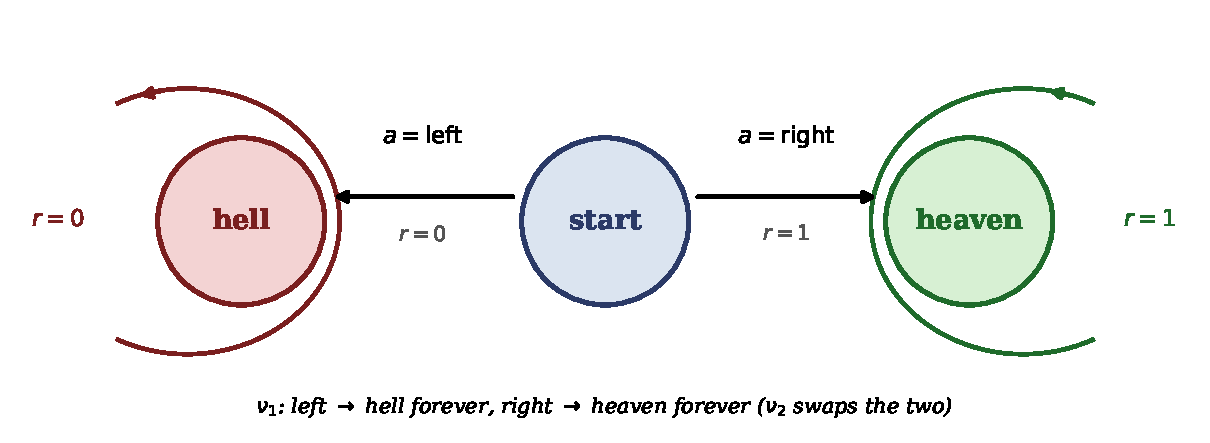
\includegraphics[width=\textwidth]{heaven_hell}
    \end{column}
  \end{columns}

  \bigskip
  No policy can be $\nu_1$-optimal \emph{and} $\nu_2$-optimal
  simultaneously. The best compromise is a random policy
  $\tilde\pi(\epsilon) = \tfrac12$ (choose either action with probability
  one half), which achieves $V^{\tilde\pi}_{\nu_i} = \tfrac12 < 1 =
  V^*_{\nu_i}$ for either $i$. That is, for $\varepsilon < \tfrac12$, no
  policy can be $\varepsilon$-optimal in $\nu_1$ and $\nu_2$
  simultaneously. \hfill$\blacklozenge$
\end{frame}

\begin{frame}[fragile]{Python: Heaven-Hell Value Computation}
  Three policies (always-left, always-right, fair coin-flip
  $\tilde\pi(\tfrac12)$) evaluated in both $\nu_1$ and $\nu_2$, using
  per-step reward as the value.

\begin{lstlisting}[style=pythonstyle]
# reward(action, env): nu1: left=0,right=1;  nu2: left=1,right=0
reward = {("left","nu1"):0.0, ("right","nu1"):1.0,
          ("left","nu2"):1.0, ("right","nu2"):0.0}

def value(p, env):   # p = {"left": prob_left, "right": prob_right}
    return sum(pr * reward[(a, env)] for a, pr in p.items())

policies = {"pi*_nu1 (right)": {"left":0.0,"right":1.0},
            "pi*_nu2 (left)":  {"left":1.0,"right":0.0},
            "fair coin":       {"left":0.5,"right":0.5}}

for name, pol in policies.items():
    v1, v2 = value(pol,"nu1"), value(pol,"nu2")
    print(f"{name:16s} V_nu1={v1:.2f} V_nu2={v2:.2f} min={min(v1,v2):.2f}")
\end{lstlisting}

  \textbf{Output.} \texttt{pi*\_nu1}: $V_{\nu_1}=1,V_{\nu_2}=0$;
  \texttt{pi*\_nu2}: $V_{\nu_1}=0,V_{\nu_2}=1$; \texttt{fair coin}:
  $V_{\nu_1}=V_{\nu_2}=0.5$ -- best worst-case value, so
  $\varepsilon<\tfrac12$ is unattainable in both simultaneously.
\end{frame}

% -----------------------------------------------------------------------------
\subsection{8.1.2 Asymptotic Optimality}
% -----------------------------------------------------------------------------

\begin{frame}[allowframebreaks]{8.1.2 Asymptotic Optimality: The Basic Idea}
  At an abstract level, an agent is \emph{asymptotically optimal} if it
  eventually (asymptotically, i.e.\ as $t\to\infty$) performs optimally.
  Mathematically, the value of the agent's policy must converge to the value
  of the optimal agent, and importantly, this convergence must hold for
  \emph{every} environment $\mu$ in the considered class $\mathcal{M}$.

  \begin{block}{Definition 8.1.4 (Asymptotic optimality)}
    A policy $\pi$ is \emph{asymptotically optimal} in an environment class
    $\mathcal{M}$ iff for all $\mu\in\mathcal{M}$, the difference between the
    optimal value function $V_\mu^*(h_{<t})$ and the value function under
    the policy $\pi$, $V_\mu^\pi(h_{<t})$, converges to zero as
    $t\to\infty$, i.e.,
    $$V_\mu^*(h_{<t}) - V_\mu^\pi(h_{<t}) \;\to\; 0 \quad \text{for } t\to\infty
    \quad \text{a.s.} \mid \text{i.p.} = \text{i.m.} \mid \text{Ces\`aro}$$
    on histories drawn from $\mu^\pi$.
  \end{block}
  \explain{$\mathcal{M}$ is a whole \textbf{class} of possible environments
    (not just one); $\mu^\pi$ means the history $h_{<t}$ is generated by
    running policy $\pi$ inside environment $\mu$; ``a.s.'' = almost surely,
    ``i.p.'' = in probability, ``i.m.'' = in mean, and ``Ces\`aro'' refers to
    convergence of the running average -- four different senses in which the
    gap can shrink to zero, discussed below.}

  \bigskip
  This is the \emph{on-policy} version of \textbf{self-optimizingness}
  (Definition 7.3.3), where the future policy $\tilde\pi$ matches the
  historic policy $\pi$ -- the histories $h_{<t}$ are distributed according
  to $\mu^\pi$ itself, i.e. the agent evaluates its own trajectory.
\end{frame}

\begin{frame}[allowframebreaks]{Four Flavours of Convergence}
  \begin{itemize}
    \item When convergence is \textbf{almost sure} (a.s.), it is called
      \textbf{strong asymptotic optimality}.
    \item When convergence is \textbf{in mean} or \textbf{in probability}
      (i.p.), it is called \textbf{asymptotic optimality in mean/probability}.
    \item When convergence is in \textbf{Ces\`aro average} (the running
      time-average of the gap goes to zero, even if the gap itself does not),
      it is called \textbf{weak asymptotic optimality}.
  \end{itemize}

  \bigskip
  Since the logical implications between modes of probabilistic convergence
  are preserved (Figure 2.8 of the book), \textbf{strong} asymptotic
  optimality implies asymptotic optimality in mean, in probability, and also
  weak asymptotic optimality. The diagram below summarizes the hierarchy
  (Section 8.1.4's Theorem 8.1.13 connects the bottom of the hierarchy to
  regret).

  \begin{center}
    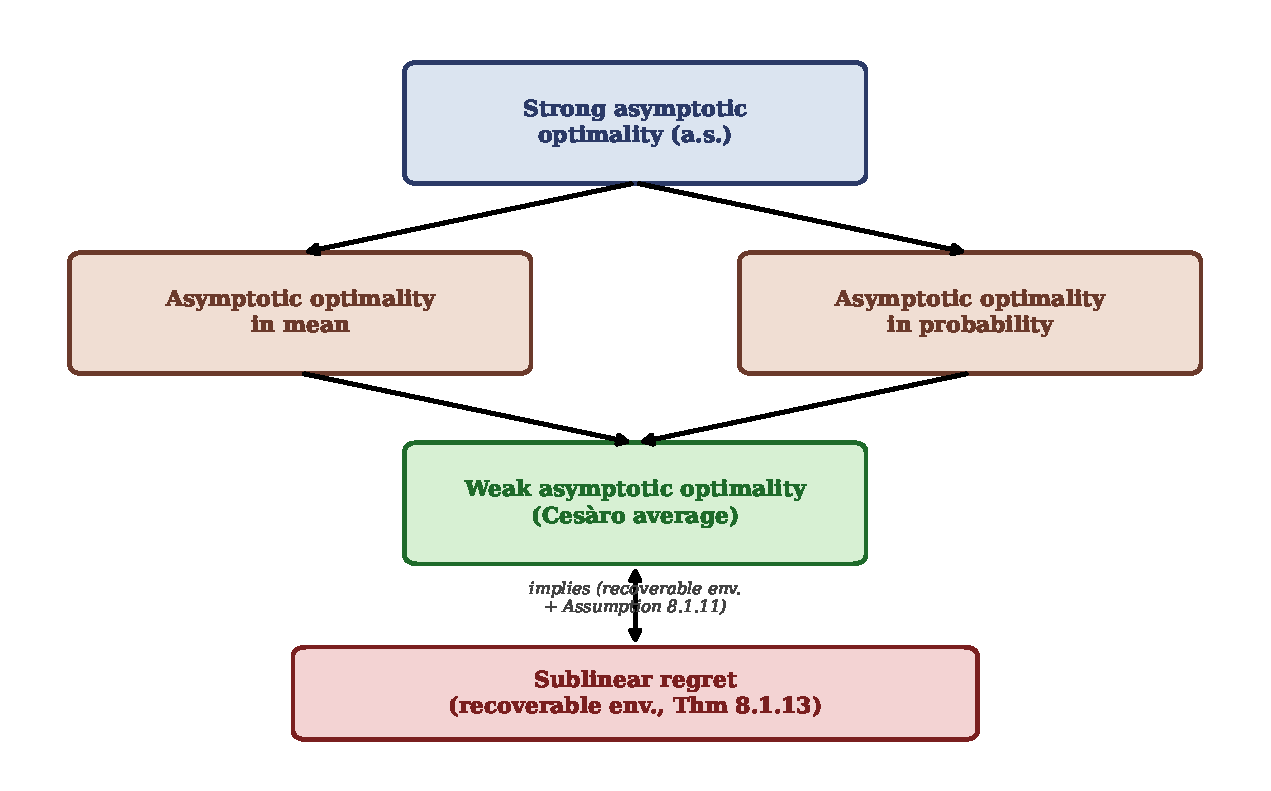
\includegraphics[width=0.62\textwidth]{optimality_hierarchy}
  \end{center}
\end{frame}

\begin{frame}{Weak Asymptotic Optimality}
  The first (weakest, and hence easiest to satisfy) asymptotic-optimality
  notion we define carefully is \textbf{weak asymptotic optimality}: an
  agent is weakly asymptotically optimal if its value function converges to
  the optimal value function \emph{on average}, i.e., convergence in
  \emph{Ces\`aro mean}.

  \begin{block}{Definition 8.1.5 (Weak asymptotic optimality)}
    A policy $\pi$ is weakly asymptotically optimal in an environment class
    $\mathcal{M}$ iff for all $\mu\in\mathcal{M}$,
    $$\mathbb{P}_\mu^\pi\left(\lim_{n\to\infty}\frac1n\sum_{t=1}^n
    \left[V_\mu^*(h_{<t}) - V_\mu^\pi(h_{<t})\right] = 0\right) = 1.$$
  \end{block}
  \explain{$\mathbb{P}_\mu^\pi(\cdot)$ is the probability under running
    policy $\pi$ in environment $\mu$; the inner sum $\frac1n\sum_{t=1}^n[
    \cdots]$ is the \textbf{running average} (over the first $n$ time steps)
    of the instantaneous value gap; requiring this average -- rather than
    each individual gap -- to vanish means the agent may make an
    \emph{infinite} number of errors, so long as they become rare enough
    that the average error washes out.}

  \bigskip
  This means the agent may make infinitely many errors while interacting
  with the environment, so long as the average number of errors is not too
  high -- the agent will still be weakly asymptotically optimal.
\end{frame}

\begin{frame}{Asymptotic Optimality in Probability / Mean}
  Convergence in probability and convergence in mean are, in general,
  \emph{separate} concepts. However, since the difference in value
  functions, $V_\mu^*(h_{<t}) - V_\mu^\pi(h_{<t})$, is always bounded
  (by $1$, since rewards lie in $[0,1]$) and non-negative (by definition of
  $V_\mu^*$ as the supremum), asymptotic optimality in probability and in
  mean turn out to be \textbf{equivalent} here.

  \begin{block}{Definition 8.1.6 (Asymptotic optimality in probability/mean)}
    A policy $\pi$ is asymptotically optimal in probability (or mean) in an
    environment class $\mathcal{M}$ iff for all $\mu\in\mathcal{M}$,
    $$\lim_{t\to\infty}\mathbf{E}_\mu^\pi\left[V_\mu^*(h_{<t}) - V_\mu^\pi(h_{<t})\right] = 0.$$
  \end{block}
  \explain{$\mathbf{E}_\mu^\pi[\cdot]$ is the expectation over histories
    generated by $\pi$ acting in $\mu$; unlike the Ces\`aro-average
    criterion above, here the \emph{individual} (not averaged) expected gap
    at time $t$ must itself vanish as $t\to\infty$ -- a strictly stronger
    requirement than weak asymptotic optimality.}
\end{frame}

\begin{frame}{Strong Asymptotic Optimality}
  \begin{block}{Definition 8.1.7 (Strong asymptotic optimality)}
    A policy $\pi$ is strongly asymptotically optimal in an environment
    class $\mathcal{M}$ iff for all $\mu\in\mathcal{M}$,
    $$\mathbb{P}_\mu^\pi\Big(\lim_{t\to\infty}\big(V_\mu^*(h_{<t}) - V_\mu^\pi(h_{<t})\big)=0\Big) = 1.$$
  \end{block}
  \explain{This is the strongest of the four notions: the value gap must
    converge to zero \emph{almost surely} along (essentially) every
    trajectory generated by $\pi$ in $\mu$ -- not just on average, and not
    just in expectation.}

  \bigskip
  As mentioned, strong asymptotic optimality is the \emph{on-policy} version
  of self-optimizingness. If in Theorem 7.3.6 we choose the historic policy
  to be the Bayes-optimal policy $\pi=\pi_\xi^*$ itself, then the conclusion
  of Theorem 7.3.6 is precisely that $\pi_\xi^*$ is strongly asymptotically
  optimal -- \emph{provided} the theorem's other conditions hold. As we will
  see in Section 8.3, achieving strong asymptotic optimality in general is
  exceedingly hard, and in some cases impossible.
\end{frame}

% -----------------------------------------------------------------------------
\subsection{8.1.3 Bayesian Optimality}
% -----------------------------------------------------------------------------

\begin{frame}{8.1.3 Bayesian Optimality}
  Considered by many to be the most reasonable definition of optimality,
  \textbf{Bayesian optimality} is optimality with respect to a
  \textbf{Bayesian mixture} over a class of environments -- rather than
  requiring optimality in one specific (and possibly unknown) environment.

  \begin{block}{Definition 8.1.8 (Bayesian optimality)}
    A policy $\pi$ is \emph{Bayes-optimal} with respect to prior
    $\{w_\nu\}$ over environment class $\mathcal{M}$ if for all histories
    $h_{<t}\in\mathcal{H}$,
    $$V_{\xi_w}^\pi(h_{<t}) = V_{\xi_w}^*(h_{<t})$$
    where $\xi_w$ is the Bayesian mixture over $\mathcal{M}$ with prior
    $\{w_\nu\}$ (Definitions 7.2.1 and 7.2.2).
  \end{block}
  \explain{$w_\nu$ is the \textbf{prior weight} the agent assigns to
    environment $\nu$ before seeing any data (all $w_\nu$ sum to $1$);
    $\xi_w$ (xi) is the resulting \textbf{Bayesian mixture} -- a single
    ``blended'' environment that behaves like a weighted average of every
    $\nu\in\mathcal{M}$; being Bayes-optimal simply means being
    $\xi_w$-optimal in the sense of Definition 8.1.1.}

  \bigskip
  \textbf{Key instances.} The agent \textbf{AIXI} is Bayes-optimal in the
  class $\Msol$ (all lower semi-computable semimeasures) with the universal
  prior $w_\nu = 2^{-K(\nu)}$; any agent maximizing \textbf{Legg-Hutter
  intelligence} (Definition 16.7.1) is also Bayes-optimal.
\end{frame}

\begin{frame}{Bayes-Optimality: The Best of Both Worlds}
  When choosing an optimality criterion, one must be very clear about
  \emph{what} behaviour is wanted, and \emph{on what timescale}. Asymptotic
  criteria only guarantee good performance \emph{eventually} -- but possibly
  not before the heat-death of the universe. Regret minimization (Section
  8.1.4) works well in the \emph{short term}, but can have undesirable
  long-run behaviour.

  \bigskip
  \textbf{Bayes-optimality can have the best of both worlds:} under certain
  conditions Bayes-optimal agents provably perform well
  \emph{asymptotically} (Theorems 7.3.1 and 7.3.6), and under the right
  choice of prior, Bayes-optimal agents can \emph{also} perform well in the
  short term.

  \bigskip
  \textbf{Equivalence to $\xi_w$-optimality.} Bayes-optimality is exactly
  $\xi_w$-optimality, a special case of $\nu$-optimality (Definition 8.1.1)
  applied to the mixture $\xi_w$ itself. The dependency of the definition on
  the prior $w$ and class $\mathcal{M}$ cannot easily be avoided:
  \begin{itemize}
    \item \textbf{Weakening} the requirement (existence of \emph{some}
      $(w,\mathcal{M})$ making $\pi$ Bayes-optimal) fails: any policy
      becomes Bayes-optimal simply by choosing a trivial environment
      $\nu_{easy}$ where every policy gets reward $1$ regardless of action,
      and setting $\mathcal{M}=\{\nu_{easy}\}$.
    \item \textbf{Strengthening} the requirement (Bayes-optimal for
      \emph{every} choice of $(w,\mathcal{M})$) also fails: given any $\pi$,
      one can construct an \emph{adversarial} environment $\nu_\pi$ that
      punishes exactly the action $\pi$ would take. No policy can then be
      Bayes-optimal for every prior, so the strengthened definition is
      useless.
  \end{itemize}
\end{frame}

\begin{frame}{Choosing a Good Prior}
  Bayes-optimality is therefore only \emph{possible} relative to some
  $(w,\mathcal{M})$, and only \emph{interesting} for ``interesting'' choices
  of $\mathcal{M}$ and $w$ -- with the pair
  $\big(2^{-K(\nu)},\;\Msol\big)$ being the most interesting choice from an
  AGI perspective.

  \bigskip
  Relying on a prior and model class can be a downside, in the sense that
  the optimality criterion depends (possibly heavily) on the choice of prior
  -- under different priors, the optimal agent may behave quite differently.
  Section 8.2 will show that there exist priors that cause a Bayes-optimal
  agent to act in undesirable ways.

  \bigskip
  On the other hand, there are good classes and priors for which
  Bayes-optimal policies \emph{are} self-optimizing (Figure 7.1 in the
  book). The most promising choice is the \textbf{universal prior}
  $2^{-K_U(\nu)}$, based on a \emph{natural} universal Turing machine $U$.
  This pushes the problem to finding a good \emph{natural} Turing machine --
  a question we return to later in the book.
\end{frame}

% -----------------------------------------------------------------------------
\subsection{8.1.4 Regret Minimization}
% -----------------------------------------------------------------------------

\begin{frame}{8.1.4 Regret Minimization}
  In hindsight it is sometimes easy to look back and see what would have
  been the best course of action -- there are many circumstances where
  optimal choices only become known \emph{after} the fact. The mathematical
  form of this notion is called \textbf{regret}.

  \begin{block}{Definition 8.1.9 (Regret)}
    The \emph{regret} of a policy $\pi$ in an environment $\mu$ with
    horizon $m$ is
    $$\mathrm{Regret}_m(\pi,\mu) := \sup_{\pi'}\mathbf{E}_\mu^{\pi'}
    \Big[\sum_{t=1}^m r_t\Big] - \mathbf{E}_\mu^\pi\Big[\sum_{t=1}^m r_t\Big]
    = m\Big[\sup_{\pi'}V_{\mu,\gamma=1}^{\pi',m}(\epsilon) - V_{\mu,\gamma=1}^{\pi,m}(\epsilon)\Big]$$
  \end{block}
  \explain{$m$ is the (finite) \textbf{horizon} -- how many time steps we
    look ahead; $\sup_{\pi'}\mathbf{E}_\mu^{\pi'}[\sum_{t=1}^m r_t]$ is the
    best possible \emph{total} expected reward over $m$ steps, achieved by
    some best competing policy $\pi'$; the second term is what $\pi$ itself
    achieves; regret is simply the \textbf{shortfall} between the two,
    rescaled by $m$ to convert the (unnormalized, undiscounted) value into
    per-step units in the rightmost expression.}

  \bigskip
  A policy has \textbf{sublinear regret} if $\mathrm{Regret}_m(\pi,\mu) =
  o(m)$, i.e., regret grows strictly slower than the horizon $m$ itself.
\end{frame}

\begin{frame}{Regret vs.\ Asymptotic Optimality}
  Since we consider the finite-horizon, unnormalized, undiscounted value
  ($\gamma_k=\llbracket k\le m\rrbracket$), the regret can be at most
  $mr_{\max}=m$. While regret is a \emph{performance measure} of the
  agent, sublinear regret is a \emph{notion of optimality}: an agent has
  sublinear regret if it does not take suboptimal actions too often.

  \bigskip
  Although it seems desirable to be as close to optimal as possible, regret
  minimization has a downside: it makes the agent not care about the long
  term, since it only cares about value up to horizon $m$ -- almost the
  \emph{exact opposite} problem to asymptotic optimality (which cares only
  about the long run, and never about the near term).

  \begin{block}{Example 8.1.10 (Regret is stronger than asymptotic optimality)}
    Consider an agent $\pi$ in an environment $\mu$ that takes the
    \emph{least rewarding} action for the first $m$ steps, then performs the
    $\mu$-optimal action on every step afterward. Measuring performance by
    regret with horizon $m$, this agent is \emph{as far from optimal as
    possible}. However, since it takes $\mu$-optimal actions after a finite
    time, it is asymptotically optimal. $\blacklozenge$
  \end{block}

  \bigskip
  This duality between regret minimization and asymptotic optimality has
  sparked research into combining the two into a single criterion.
\end{frame}

\begin{frame}[fragile]{Python: Sublinear vs.\ Linear vs.\ Finite Regret}
  Three qualitatively different regret behaviours: never learning (linear),
  a reasonable learner (sublinear), and Example 8.1.10's agent (finite regret).

  \begin{columns}
    \begin{column}{0.56\textwidth}
\begin{lstlisting}[style=pythonstyle]
import numpy as np
m = np.arange(1, 201)
linear    = 0.5*m               # never learns
sublinear = 3.0*np.sqrt(m)      # o(m)
finite    = 8.0*(1-np.exp(-m/15))  # Ex. 8.1.10

for name, r in [("linear", linear),
                ("sublinear", sublinear),
                ("finite", finite)]:
    ratio = r[-1] / m[-1]  # -> 0 iff sublinear
    print(f"{name:9s} R_200={r[-1]:6.2f} ratio={ratio:.3f}")
\end{lstlisting}
    \end{column}
    \begin{column}{0.42\textwidth}
      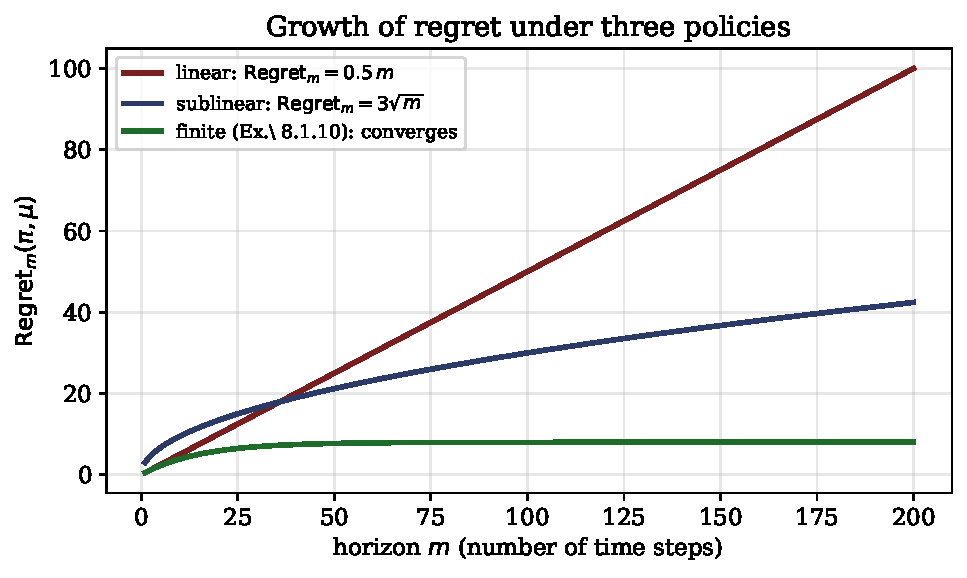
\includegraphics[width=\textwidth]{regret_curves}
    \end{column}
  \end{columns}

  \textbf{Output.} \texttt{linear}: ratio$=0.500$ (does not vanish);
  \texttt{sublinear}: ratio$=0.212$ (shrinking, i.e.\ $o(m)$);
  \texttt{finite}: ratio$\approx0.040$, shrinking fastest.
\end{frame}

\begin{frame}[allowframebreaks]{Assumptions Needed to Connect Regret and Asymptotic Optimality}
  \begin{block}{Assumption 8.1.11 (Extra discount function assumptions)}
    Let the discount function $\gamma$ (gamma) be such that
    \begin{itemize}
      \item $\gamma_t > 0$ for all $t$;
      \item $\gamma_t$ is decreasing in $t$;
      \item $\lim_{t\to\infty} H_t(\varepsilon)/t = 0$ for all $\varepsilon>0$;
    \end{itemize}
    where $H_t(\varepsilon)$ is the \emph{effective horizon} (Definition 6.4.2).
  \end{block}
  \explain{The first bullet says a positive reward is still worth
    \emph{something} no matter how far in the future; the second says
    rewards closer to the present are always worth at least as much as
    rewards received later; the third bounds how far-sighted the
    $\varepsilon$-effective horizon $H_t(\varepsilon)$ (roughly: how many
    future steps still matter) is allowed to be, relative to $t$ itself.
    \textbf{Geometric discounting} satisfies all three.}

  \bigskip
  We also need to restrict to environments the agent can \emph{recover}
  from mistakes in -- a form of \emph{ergodicity} assumption, since an agent
  exploring an environment it believes is safe may take an action (``fall
  off a cliff'') from which it can never learn to stop repeating.

  \bigskip
  Let $\mathbf{E}_{\nu_1}^{\pi_1}[V_{\nu_2}^{\pi_2}(h_{<t})]$ denote the
  expected value function of policy $\pi_2$ on environment $\nu_2$, given a
  past history $h_{<t}$ generated by policy $\pi_1$ on environment $\nu_1$.
\end{frame}

\begin{frame}{Recoverable Environments}
  \begin{block}{Definition 8.1.12 (Recoverable environments)}
    An environment $\mu$ is \emph{recoverable} iff
    $$\sup_\pi \Big|\mathbf{E}_{\mu}^{\pi_\mu^*}\big[V_\mu^*(h_{<t})\big] -
    \mathbf{E}_\mu^\pi\big[V_\mu^*(h_{<t}')\big]\Big| \longrightarrow 0
    \quad \text{for } t\to\infty$$
  \end{block}
  \explain{Note the expectations are with respect to \emph{different}
    policies: the history $h_{<t}$ is sampled from running the optimal
    policy $\pi_\mu^*$, whereas $h_{<t}'$ is sampled from running an
    arbitrary policy $\pi$. Intuitively, \textbf{recoverable} means that no
    matter what the past history was, or how poor a policy $\pi$ was
    followed, \emph{switching} to an optimal policy $\pi^*$ from time $t$
    onward converges to the same value as if the optimal policy had been
    followed from the very beginning.}

  \bigskip
  This means that no action can permanently lock the agent out of parts of
  the environment needed for maximum reward, and any early mistakes can be
  recovered from -- this excludes things like cliffs one cannot climb back
  from, and traps such as the Heaven-Hell environment (Example 8.1.3), where
  taking \emph{left} once locks the agent into hell forever.
\end{frame}

\begin{frame}{Theorem 8.1.13: Sublinear Regret in Recoverable Environments}
  \begin{block}{Theorem 8.1.13 (Sublinear regret in recoverable environments)}
    If the discount function $\gamma$ satisfies Assumption 8.1.11, the
    environment $\mu$ is recoverable, and $\pi$ is asymptotically optimal in
    mean in $\mathcal{M}=\{\mu\}$, then $\mathrm{Regret}_m(\pi,\mu) = o(m)$.
  \end{block}
  \explain{In words: if the discount is well-behaved, the environment lets
    you recover from mistakes, and your policy is asymptotically optimal in
    mean (Definition 8.1.6), then your policy is \emph{automatically}
    guaranteed to have sublinear regret. This is one concrete way of
    combining the ``short-term'' regret criterion with the ``long-term''
    asymptotic-optimality criterion.}

  \bigskip
  This connects the middle of the hierarchy figure shown earlier
  (asymptotic optimality in mean) to sublinear regret at the bottom, under
  the recoverability and discount assumptions. The full proof (next slides)
  is a careful bookkeeping argument combining the triangle inequality with
  properties of the effective horizon.
\end{frame}

\begin{frame}[allowframebreaks]{Proof of Theorem 8.1.13}
  We follow the proof from [Lei16b]. Let $\pi_m := \arg\max_\pi
  \mathrm{Regret}_m(\pi,\mu)$. We want to show that
  $$\limsup_{m\to\infty}\mathbf{E}_\mu^{\pi_m}\Big[\frac1m\sum_{t=1}^m r_t\Big]
  - \mathbf{E}_\mu^\pi\Big[\frac1m\sum_{t=1}^m r_t\Big] \le 0.$$

  Let $d_k^{(m)} := \mathbf{E}_\mu^{\pi_m}[r_k] - \mathbf{E}_\mu^\pi[r_k]$.
  We have $-1\le d_k^{(m)}\le 1$, since rewards are bounded between $0$ and
  $1$. From the definition of \emph{recoverable}, since $\pi$ and $\pi_m$
  are not worse than the worst policy, we have that
  $$\Big|\mathbf{E}_\mu^{\pi_\mu^*}[V_\mu^*(h_{<t})] - \mathbf{E}_\mu^\pi[V_\mu^*(h_{<t})]\Big| \to 0
  \quad\text{and}\quad
  \sup_m\Big|\mathbf{E}_\mu^{\pi_\mu^*}[V_\mu^*(h_{<t})] - \mathbf{E}_\mu^{\pi_m}[V_\mu^*(h_{<t})]\Big| \to 0$$
  for $t\to\infty$. Combining these with the triangle inequality we get
  \begin{equation*}
  \sup_m \mathbf{E}_\mu^{\pi_m}[V_\mu^*(h_{<t})] - \mathbf{E}_\mu^\pi[V_\mu^*(h_{<t})] \to 0
  \quad \text{for } t\to\infty. \tag{8.1.14}
  \end{equation*}

  Since $\pi$ is asymptotically optimal in mean we have that
  $$\mathbf{E}_\mu^\pi[V_\mu^*(h_{<t})] - \mathbf{E}_\mu^\pi[V_\mu^\pi(h_{<t})] \to 0 \quad \text{for } t\to\infty.$$
  Combining the two previous lines we get
  $$\sup_m \mathbf{E}_\mu^{\pi_m}[V_\mu^*(h_{<t})] - \mathbf{E}_\mu^\pi[V_\mu^\pi(h_{<t})] \to 0 \quad \text{for } t\to\infty.$$
  Since $V_\mu^* \ge V_\mu^{\pi_m}$ we have
  \begin{equation*}
  \limsup_{t\to\infty}\Big[\sup_m \mathbf{E}_\mu^{\pi_m}[V_\mu^{\pi_m}(h_{<t})] - \mathbf{E}_\mu^\pi[V_\mu^\pi(h_{<t})]\Big] \le 0. \tag{8.1.15}
  \end{equation*}

  \framebreak

  For any policy $\pi'$ we can rewrite our expectation of the value function as
  $$E_\mu^{\pi'}[V_\mu^{\pi'}(h_{<t})] = \mathbf{E}_\mu^{\pi'}\Big[\frac1{\Gamma_t}\sum_{k=t}^\infty \gamma_k r_k\Big]
  = \frac1{\Gamma_t}\sum_{k=t}^\infty \gamma_k \mathbf{E}_\mu^{\pi'}[r_k]$$
  Then, using this form for (8.1.14) and (8.1.15) and $d_k^{(m)}$, we get
  $$\limsup_{t\to\infty}\sup_m \frac1{\Gamma_t}\sum_{k=t}^\infty \gamma_k d_k^{(m)} \le 0.$$

  Let $\varepsilon>0$. Choose $t_0$ independent of $m$ and large enough
  such that $\frac1{\Gamma_t}\sum_{k=t}^\infty \gamma_k d_k^{(m)} < \varepsilon$
  for all $m$ and $t\ge t_0$. We split $\sum_{k=1}^m d_k^{(m)}$ at $t_0$, and
  define $b_t$ for $t_0\le t\le m$ as
  $$b_{t_0} = \frac{\Gamma_{t_0}}{\gamma_{t_0}} \qquad\text{and}\qquad
  b_t = \frac{\Gamma_t}{\gamma_t} - \frac{\Gamma_t}{\gamma_{t-1}} \quad \text{for } t>t_0.$$
  The following equalities for $b_t$ can be verified by inserting the
  definitions and swapping the two sums:
  \begin{equation*}
  \sum_{t=t_0}^m d_t^{(m)} = \sum_{t=t_0}^m \frac{b_t}{\Gamma_t}\sum_{k=t}^m \gamma_k d_k^{(m)}
  \qquad\text{and}\qquad \sum_{t=t_0}^m \frac{b_t}{\Gamma_t} = \frac1{\gamma_m}. \tag{8.1.16}
  \end{equation*}

  \framebreak

  Additionally, for the sum from $t_0$ to $m$ of $b_t$ we get
  $$\sum_{t=t_0}^m b_t = \frac{\Gamma_{t_0}}{\gamma_{t_0}} + \sum_{t=t_0+1}^m
  \Big(\frac{\Gamma_t}{\gamma_t}-\frac{\Gamma_t}{\gamma_{t-1}}\Big)
  = \frac{\Gamma_{m+1}}{\gamma_m} + m - t_0 + 1$$
  From the definition of the effective horizon $H_m(\varepsilon)$
  (Definition 6.4.2) and the monotonicity assumption on $\gamma$ we get
  \begin{align*}
  \varepsilon\Gamma_m &\ge \Gamma_{m+H_m(\varepsilon)} = \Gamma_m - \gamma_m -
  \cdots - \gamma_{m+H_m(\varepsilon)-1} \ge \Gamma_m - H_m(\varepsilon)\gamma_m \\
  \text{which implies}&\quad \frac{H_m(\varepsilon)}{1-\varepsilon} \ge
  \frac{\Gamma_m}{\gamma_m} \ge \frac{\Gamma_{m+1}}{\gamma_m}.
  \end{align*}

  Combining everything we get for the regret
  \footnotesize
  \begin{align*}
    \mathrm{Regret}_m(\pi,\mu) &= \sum_{t=1}^m d_t^{(m)}
    \le t_0 + \sum_{t=t_0}^m b_t \frac1{\Gamma_t}\sum_{k=t}^m \gamma_k d_k^{(m)} \\
    &\le t_0 + \sum_{t=t_0}^m b_t \frac1{\Gamma_t}\sum_{k=t}^\infty \gamma_k d_k^{(m)}
       - \sum_{t=t_0}^m \frac{b_t}{\Gamma_t}\sum_{k=m+1}^\infty \gamma_k d_k^{(m)} \\
    &< t_0 + \sum_{t=t_0}^m b_t\varepsilon + \sum_{t=t_0}^m \frac{b_t \Gamma_{m+1}}{\Gamma_t} \\
     &= t_0 + \varepsilon\frac{\Gamma_{m+1}}{\gamma_m} + \varepsilon(m-t_0+1) + \frac{\Gamma_{m+1}}{\gamma_m} \\
    &\le t_0 + \frac{(1+\varepsilon)H_m(\varepsilon)}{1-\varepsilon} + \varepsilon(m-t_0+1)
  \end{align*}
  \normalsize
  By Assumption 8.1.11 we have $H_m(\varepsilon)=o(m)$, hence
  $$\limsup_{m\to\infty}\frac1m\mathrm{Regret}_m(\pi,\mu) \le \varepsilon.$$
  Since $\varepsilon$ was arbitrary, we have the desired result. $\blacksquare$
\end{frame}

% -----------------------------------------------------------------------------
\subsection{8.1.5 Pareto Optimality}
% -----------------------------------------------------------------------------

\begin{frame}[allowframebreaks]{8.1.5 Pareto Optimality}
  Related to the game-theoretic notion of \textbf{Pareto Efficiency}, an
  agent is \emph{Pareto optimal} if there is no other agent which is at
  least as good in \emph{every} environment, and strictly better in
  \emph{at least one}.

  \begin{block}{Definition 8.1.17 (Pareto optimality)}
    A policy $\pi$ is Pareto optimal in a set of environments $\mathcal{M}$
    iff there is no policy $\pi'$ such that $V_\nu^{\pi'}\ge V_\nu^\pi$ for
    all $\nu\in\mathcal{M}$ and $V_\rho^{\pi'} > V_\rho^\pi$ for at least
    one $\rho\in\mathcal{M}$.
  \end{block}
  \explain{$\pi'$ ``dominates'' $\pi$ if it never does worse in \emph{any}
    environment $\nu\in\mathcal{M}$, and does strictly better in
    \emph{at least one} environment $\rho\in\mathcal{M}$; $\pi$ is Pareto
    optimal exactly when no such dominating $\pi'$ exists.}

  \bigskip
  Pareto optimality is useful when there is a \emph{set of conflicting
  criteria} we want to be optimal in simultaneously -- here, the different
  criteria are performance in the different environments $\nu\in\mathcal{M}$.
  The set of Pareto-optimal agents is called the \textbf{Pareto frontier}.

  \begin{center}
    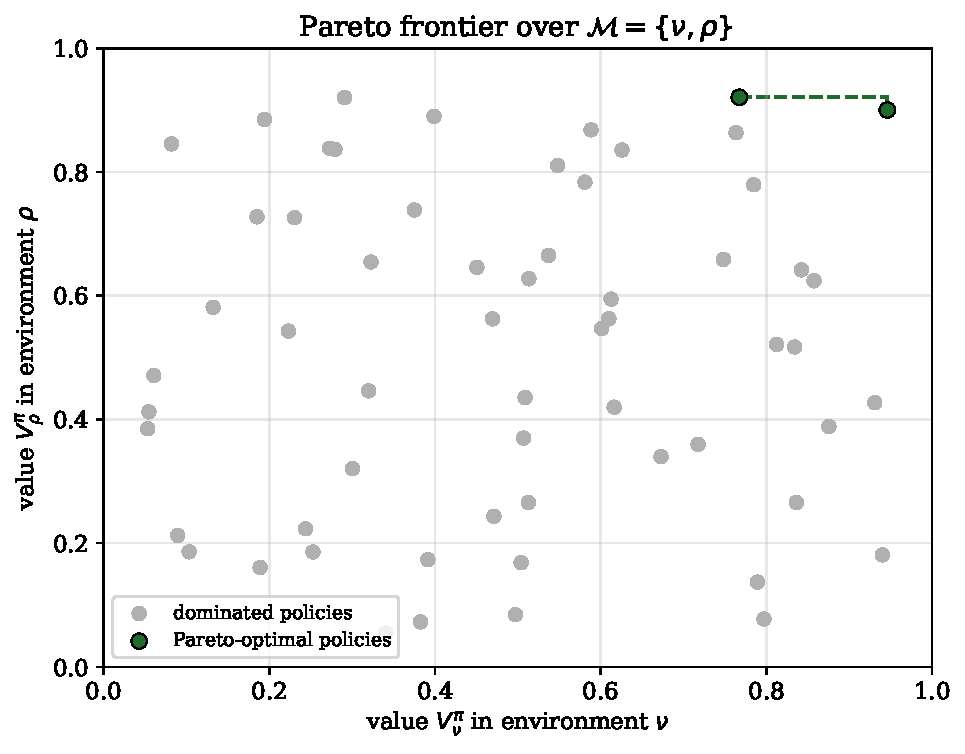
\includegraphics[width=0.42\textwidth]{pareto_frontier}
  \end{center}
\end{frame}

\begin{frame}[allowframebreaks]{Theorem 8.1.18: AI$\xi$ and AIXI Are Pareto Optimal}
  \begin{block}{Theorem 8.1.18 (AI$\xi$ and AIXI are Pareto optimal)}
    The Bayes-optimal policy $\pi_\xi^*$ (and in particular AIXI, its
    special case with $\mathcal{M}=\Msol$) is Pareto optimal.
  \end{block}

  \textbf{Proof.} Assume $\pi_\xi^*$ is \emph{not} Pareto optimal, and let
  $\pi$ be a dominating policy, i.e.\ $V_\nu^\pi \ge V_\nu^{\pi_\xi^*}$ for
  all $\nu\in\mathcal{M}$ with strict inequality for at least one
  $\nu\in\mathcal{M}$. Then
  $$V_\xi^\pi = \sum_\nu w_\nu V_\nu^\pi > \sum_\nu w_\nu V_\nu^{\pi_\xi^*}
  = V_\xi^{\pi_\xi^*} \equiv V_\xi^* \ge V_\xi^\pi$$
  \explain{The two equalities follow from \textbf{linearity} of $V_\rho$
    (Theorem 7.2.5, the mixture value is a weighted sum of the individual
    values); the strict inequality follows from the domination assumption
    and $w_\nu>0$ for all $\nu$; the last inequality follows because
    $\pi_\xi^*$ \emph{maximizes} value under the mixture $\xi$ by
    definition. The chain gives $V_\xi^\pi > V_\xi^\pi$ -- a contradiction --
    proving Pareto optimality of $\mathrm{AI}\xi$. AIXI is the special case
    of $\mathrm{AI}\xi$ with $\mathcal{M}=\Msol$.} $\blacksquare$

  \bigskip
  It is comforting that $\mathrm{AI}\xi$ is Pareto optimal, since a
  violation would clearly render $\pi_\xi^*$ intuitively suboptimal.
  Unfortunately, for any class of environments containing $\Mcomp$ (all
  computable environments), \emph{every} policy is Pareto optimal [Lei16b] --
  so Pareto optimality becomes a \textbf{vacuous} notion for AIXI.
\end{frame}

\begin{frame}[allowframebreaks]{Theorem 8.1.19: Pareto Optimality Becomes Vacuous}
  \begin{block}{Theorem 8.1.19 (Every policy is Pareto optimal in any $\mathcal{M}\supseteq\Mcomp$)}
    If $\mathcal{M}\supseteq\Mcomp$ (contains all computable
    environments), then every policy $\pi$ is Pareto optimal in $\mathcal{M}$.
  \end{block}

  \textbf{Proof (sketch).} [Lei16b] Assume for contradiction that some
  policy $\pi'$ strictly dominates $\pi$: $V_\nu^{\pi'}\ge V_\nu^\pi$ for
  all $\nu$, with strict inequality at some $\rho\in\mathcal{M}$. Since
  $V_\rho^{\pi'}>V_\rho^\pi$, there must be some history where $\pi$ and
  $\pi'$ take different actions. Let $\dot h_{<t}$ be the
  (lexicographically) \emph{first} such history, and $\dot a_t$ an action
  with $\pi(\dot a_t|\dot h_{<t}) > \pi'(\dot a_t|\dot h_{<t})$.

  \bigskip
  We can define a \emph{computable} environment $\mu$, identical to $\rho$
  for any history that is not an extension of $\dot h_{<t}$, but which
  rewards $1$ forever if action $\dot a_t$ is taken at $\dot h_{<t}$, and
  $0$ otherwise. Since $\pi$ takes $\dot a_t$ more likely than $\pi'$ given
  $\dot h_{<t}$, and they coincide otherwise, we get $V_\mu^\pi >
  V_\mu^{\pi'}$ -- contradicting that $\pi'$ dominates $\pi$, since
  $\mu\in\Mcomp\subseteq\mathcal{M}$. $\blacksquare$

  \bigskip
  \textbf{Takeaway.} In the context of Universal AI, Pareto optimality
  gives no useful information: virtually \emph{any} policy, however bad,
  satisfies it -- so we need a \emph{refined} version.
\end{frame}

\begin{frame}[allowframebreaks]{Balanced Pareto Optimality}
  \begin{block}{Definition 8.1.20 (Balanced Pareto optimality [Hut02c, Lei16b])}
    Given a prior $w\in\Delta'\mathcal{M}$ where $\mathcal{M}$ is an
    environment class, a policy $\pi$ is \emph{balanced Pareto optimal} if
    it achieves a better value across $\mathcal{M}$ \emph{weighted by}
    $w\in\Delta'\mathcal{M}$ than any other policy, formally, if for all
    policies $\tilde\pi$,
    $$\sum_{\nu\in\mathcal{M}} w_\nu\big[V_\nu^\pi - V_\nu^{\tilde\pi}\big] \ge 0.$$
  \end{block}
  \explain{Instead of demanding domination in \emph{every single}
    environment (too weak, as we saw), balanced Pareto optimality only
    requires domination in the prior-\textbf{weighted average} sense --
    exactly analogous to how Bayesian optimality relaxes $\nu$-optimality.}

  \bigskip
  All and only Bayes-optimal policies $\pi_{\xi_w}^*$ are balanced Pareto
  optimal for $w$:
  $$\sum_{\nu\in\mathcal{M}} w_\nu[V_\nu^\pi - V_\nu^{\tilde\pi}] =
  V_{\xi_w}^\pi - V_{\xi_w}^{\tilde\pi} \ge 0 \;\;\forall\tilde\pi \quad
  \text{iff} \quad \pi = \pi_{\xi_w}^*$$

  Hence balanced Pareto optimality has the \emph{same} features
  (advantages and problems) as Bayes-optimality (Section 8.1.3), e.g.\ its
  dependence on the prior. Section 8.2 describes possible bad priors that
  make balanced Pareto optimality a less useful definition.
\end{frame}

% =============================================================================
\section{8.2 Bad Priors}
% =============================================================================

\begin{frame}{8.2 Bad Priors: Overview}
  The prior is one of the most important aspects for Bayesian optimality.
  However, as we will show below, some priors are less than ideal, and can
  cause Bayes-optimal policies to perform quite poorly [Ors10, Lei16b,
  LH15b].

  \bigskip
  We consider two families of ``bad'' priors:
  \begin{itemize}
    \item the \textbf{dogmatic prior} (Section 8.2.1): makes the
      Bayes-optimal agent dogmatically follow a single, arbitrary,
      pre-chosen policy;
    \item the \textbf{indifference prior} (Section 8.2.2): makes
      \emph{every} policy Bayes-optimal, so the agent's actions are
      determined purely by an arbitrary tie-breaking rule.
  \end{itemize}
  Both priors are \emph{adversarially chosen} -- they are constructed
  specifically to cause bad behaviour, and are highly unnatural.
\end{frame}

% -----------------------------------------------------------------------------
\subsection{8.2.1 Dogmatic Prior}
% -----------------------------------------------------------------------------

\begin{frame}{8.2.1 The Dogmatic Prior}
  Given any policy and a history generated by that policy interacting with
  the environment, there is a prior for which \emph{following that policy}
  is Bayes-optimal. We call this the \textbf{dogmatic prior}, as the
  Bayes-optimal agent \emph{dogmatically} believes it must follow that
  policy. Dogmatically following a single policy will rarely be what we
  want a Bayes-optimal agent to do, since the agent will never learn from
  its mistakes -- but note the priors here are adversarially chosen.

  \begin{block}{Theorem 8.2.1 (Dogmatic prior [LH15b])}
    Let $\pi$ be any deterministic computable policy, let $\xi$ be any
    Bayesian mixture over $\Msol$ with weights $w\in\Delta'\Msol$, and let
    $\varepsilon\in\mathbb{Q}$ with $\varepsilon>0$. There is a universal
    mixture $\xi'$ with respect to some prior such that for any history
    $h_{<t}$ consistent with $\pi$ and $V_\xi^\pi(h_{<t})>\varepsilon$, the
    action $\pi(h_{<t})$ is the \emph{unique} $\xi'$-optimal action.
  \end{block}
  \explain{$\Delta'\Msol$ is the set of valid priors (probability
    distributions) over $\Msol$; the theorem says we can build a
    \emph{new} universal mixture $\xi'$ under which \emph{any} fixed
    deterministic policy $\pi$ becomes the uniquely optimal thing to do --
    for as long as $\pi$'s own value estimate stays above the threshold
    $\varepsilon$.}
\end{frame}

\begin{frame}[allowframebreaks]{Proof of Theorem 8.2.1}
  This proof follows [Lei16b]. For all environments $\nu\in\Msol$ we can
  define a \emph{new} environment $\rho_{\pi,\nu}\in\Msol$ that is
  identical to $\nu$ until it receives an action $\pi$ would \emph{not}
  take, then outputs reward $0$ forever. We derive new weights $w'$ that
  weigh environments $\rho_{\pi,\nu}$ higher than $\nu$. Define
  $$w'_\nu := \varepsilon w_\nu \;\;\text{if}\;\; \nu\ne\rho_{\pi,\nu'}\;\forall\nu'\in\Msol
  \qquad\text{and}\qquad w'_{\rho_{\pi,\nu}} := (1-\varepsilon)w_\nu + \varepsilon w_{\rho_{\pi,\nu}} \;\;\text{otherwise}$$

  Checking that the new weights sum to $1$,
  \begin{align*}
    \sum_{\nu\in\Msol} w'_\nu &= \sum_{\nu=\rho_{\pi,\nu}} w'_\nu + \sum_{\nu\ne\rho_{\pi,\nu'}\forall\nu'} w'_\nu \\
    &= \sum_{\nu=\rho_{\pi,\nu}}\big((1-\varepsilon)w_{\rho_{\pi,\nu}} + \varepsilon w_\nu\big) + \sum_{\nu\ne\rho_{\pi,\nu'}\forall\nu'} \varepsilon w_\nu \\
    &= \sum_{\nu\in\Msol}\varepsilon w_\nu + \sum_{\nu\in\Msol}(1-\varepsilon)w_\nu
    = \varepsilon + (1-\varepsilon) = 1
  \end{align*}
  Therefore $w'$ is a valid prior over $\Msol$, and we define a Bayesian
  mixture $\xi'$ using $w'$. We can also define the mixture over the
  $\rho$'s by $\rho := \sum_{\nu\in\Msol} w_\nu\rho_{\pi,\nu}$, and rewrite
  $\xi'$ as $\xi' = \varepsilon\xi + (1-\varepsilon)\rho$.

  \framebreak

  From now on, let $h_{<t}$ be a history consistent with $\pi$, i.e.\
  actions generated by $\pi$. For such $h_{<t}$, $\rho_{\pi,\nu}=\nu$, hence
  $\rho=\xi$, hence $\xi'=\xi$. Considering the class
  $\mathcal{M}=\{\xi,\rho\}$ with prior $w_\xi=\varepsilon$ and
  $w_\rho=1-\varepsilon$, this implies that the posterior coincides with
  the prior on such $h_{<t}$ (Definition 7.2.2). Linearity of the Q-value
  function (Theorem 7.2.5) for any policy $\pi'$ and action $a_t$ can hence
  be expressed in terms of prior weights
  $$Q_{\xi'}^{\pi'}(h_{<t}a_t) = \varepsilon Q_\xi^{\pi'}(h_{<t}a_t) + (1-\varepsilon)Q_\rho^{\pi'}(h_{<t}a_t)$$

  Let $a^*=\pi(h_{<t})$ and $a'$ be any other action. We show that $a^*$ is
  the $\xi'$-optimal action by showing $V_{\xi'}^*(h_{<t}a^*) >
  V_{\xi'}^*(h_{<t}a')$.
  $$Q_{\xi'}^*(h_{<t}a^*) \ge Q_{\xi'}^\pi(h_{<t}a^*) = Q_\xi^\pi(h_{<t}a^*) = V_\xi^\pi(h_{<t}) > \varepsilon$$
  $$Q_{\xi'}^*(h_{<t}a') = \varepsilon Q_\xi^\pi(h_{<t}a') + (1-\varepsilon)Q_\rho^\pi(h_{<t}a') = \varepsilon Q_\xi^\pi(h_{<t}a') + 0 \le \varepsilon$$
  Therefore $a^* = \pi(h_{<t})$ is the $\xi'$-optimal action for history
  $h_{<t}$. $\blacksquare$
\end{frame}

\begin{frame}[fragile]{Python: Dogmatic-Prior Weight Redistribution}
  Toy illustration of Theorem 8.2.1's weight redistribution: a
  $3$-environment class $w=(0.5,0.3,0.2)$, $\varepsilon=0.3$; following
  $\pi$ (consistent with $\nu_1$) traps $\nu_2,\nu_3$-mass into $\rho$.

  \begin{columns}
    \begin{column}{0.56\textwidth}
\begin{lstlisting}[style=pythonstyle]
w = {"nu1":0.5, "nu2":0.3, "nu3":0.2}
eps = 0.3
# nu1 consistent with pi -> rho=nu1 here
w_prime = {
  "rho_pi_nu1": (1-eps)*w["nu1"]+eps*w["nu1"],
  "nu2_kept":   eps*w["nu2"],
  "nu3_kept":   eps*w["nu3"],
}
trapped = (1-eps)*(w["nu2"]+w["nu3"])
print("w'      :", w_prime)
print("trapped :", round(trapped,3))
print("total   :", round(sum(w_prime.values())+trapped,3))
\end{lstlisting}
    \end{column}
    \begin{column}{0.42\textwidth}
      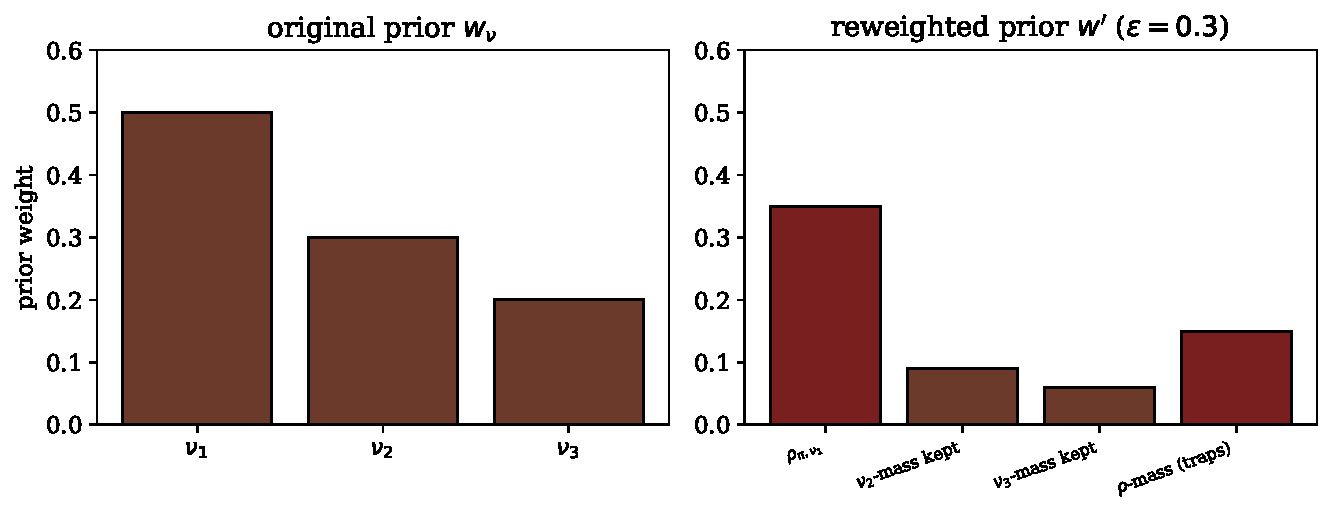
\includegraphics[width=\textwidth]{dogmatic_prior}
    \end{column}
  \end{columns}

  \textbf{Output.} $w'$ still sums to $1.0$, but now favours the
  $\pi$-consistent branch ($\rho_{\pi,\nu_1}=0.5$), while deviating from
  $\pi$ routes mass into trap environments rewarding $0$ forever.
\end{frame}

% -----------------------------------------------------------------------------
\subsection{8.2.2 Indifference Prior}
% -----------------------------------------------------------------------------

\begin{frame}{8.2.2 The Indifference Prior}
  Another bad prior is the \textbf{indifference prior}. Under certain
  conditions, this prior makes \emph{all} policies Bayes-optimal with
  respect to it. Because all policies are optimal (and therefore equal in
  value), the Bayes-optimal agent using this prior chooses its actions
  entirely based on whatever \textbf{tie-breaker} is used -- which is not
  ideal, since depending on the tie-breaker, the agent can be convinced to
  take \emph{any} arbitrary action.

  \begin{block}{Theorem 8.2.2 (Indifference prior [LH15b])}
    If there is an $m$ such that the discount normalization factor
    $\Gamma_{m+1}=0$, then there is a Bayesian mixture $\xi'$ such that
    \textbf{all} policies are $\xi'$-optimal.
  \end{block}
  \explain{$\Gamma_{m+1}$ (Gamma) is the discount normalizer for time steps
    after $m+1$ (Table 6.4); if it is exactly zero, it means \emph{nothing}
    that happens after time $m$ can affect the value function at all, so
    the mixture $\xi'$ can be constructed to render every policy's choices
    after $m$ irrelevant, while ``masking'' its earlier choices too.}

  \bigskip
  This relies heavily on the assumption that eventually $\Gamma_{m+1}$
  becomes $0$, which is never the case with the standard \textbf{geometric
  discounting} (where $\Gamma_t>0$ for all finite $t$) -- but does happen
  for finite-lifetime discounting.
\end{frame}

\begin{frame}[allowframebreaks]{Proof of Theorem 8.2.2}
  This proof follows [Lei16b]. Assume the action space is
  $\mathcal{A}=\{0,1\}$. Let $U$ be some universal Turing machine and
  define $U'$ such that $U'$ does not halt on programs of length less than
  $m$, and for programs of length greater than $m-1$,
  $$U'(p,a) := U(p_{m:\ell(p)},\, a \;\mathrm{xor}\; p_{1:\ell(a)})$$
  \explain{$\ell(p)$ is the length of program $p$; ``xor'' flips bits of the
    action according to the first $\ell(a)$ bits of the program $p$ -- so
    $U'$ reserves its first $m-1$ bits purely to \emph{mask} (via XOR) the
    actions taken, rather than using them for anything else.}

  Then we can define a chronological Solomonoff distribution (which by
  Theorem 3.8.8, extended to the agent case (7.4.9), is a Bayesian mixture
  $\xi'$) with respect to $U'$ as the underlying universal Turing machine as
  $$\xi'(e_{<m}\|a_{<m}) = \sum_{p:e_{<m}\sqsubseteq U'(p,a_{<m})} 2^{-\ell(p)}
  \overset{(a)}{=} \sum_{s_{<m}p':e_{1:t}\sqsubseteq U'(s_{<m}p',a_{<m})} 2^{-m-1-\ell(p')}$$
  $$= \sum_{s_{<m}}\sum_{p':e_{1:t}\sqsubseteq U(p',a_{<m}\;\mathrm{xor}\;s_{<m})} 2^{-m-1-\ell(p')}
  \overset{(b)}{=} \sum_{s_{<m}}\sum_{p':e_{1:t}\sqsubseteq U(p',s_{<m})} 2^{-m-1-\ell(p')}$$

  \framebreak

  Step $(a)$ comes from decomposing $p$ as $s_{<m}p$. Step $(b)$ comes from
  the fact that we are summing over \emph{all} $s_{<m}$ and xor-ing them
  with $a_{<m}$, which is identical to simply summing over all $s_{<m}$
  again (relabelling the dummy variable). Therefore the mixture $\xi'$ does
  \textbf{not} depend on $a_{<m}$ for the first $m-1$ actions.

  \bigskip
  For the remaining actions, since $\Gamma_m=0$, the rewards after time
  step $m$ do not matter. Since the mixture does not depend on the actions
  taken (for the first $m-1$ steps) and rewards after $m$ are irrelevant,
  \emph{all} policies have the same value $V_\xi^\pi$ -- hence all policies
  are optimal with respect to this mixture. $\blacksquare$

  \bigskip
  \textbf{Remark.} This example is very artificial, and not unexpected
  given the unnatural universal Turing machine $U'$, which depends on $m$
  and reserves $m-1$ bits to ``mask'' the first $m-1$ actions. If we
  increase AIXI's lifetime while fixing the UTM $U'$, the result no longer
  holds.
\end{frame}

\begin{frame}{Discussion: Solomonoff Induction Errors}
  An analogous result holds for \textbf{Solomonoff induction}: Theorem
  3.8.9 and Corollary 3.5.14 imply that Solomonoff's distribution $M$ makes
  at most
  $$K(\mu)\cdot 2\ln 2 = Km(x_{1:\infty})\cdot 2\ln 2$$
  errors for predicting deterministic sequences $x_{1:\infty}$.
  \explain{$K(\mu)$ is the Kolmogorov complexity of the true generating
    environment $\mu$; $Km(x_{1:\infty})$ is (essentially) the same
    quantity phrased in terms of the sequence's monotone complexity; $2\ln2$
    is a fixed constant coming from the error-bound proof. In words:
    Solomonoff induction makes a \emph{bounded} number of prediction errors,
    proportional to how ``complex'' (hard to compress) the true sequence is.}

  \bigskip
  In case the shortest program (for $\mu$) has length $>m$, there is
  \textbf{no guarantee} that we make fewer than $m$ errors -- so the
  indifference-prior pathology is really about the interaction between a
  \emph{finite} lifetime $m$ and an adversarially long minimal program
  length, not a failure of Solomonoff induction itself.
\end{frame}

% -----------------------------------------------------------------------------
\subsection{8.2.3 Bad Priors, Bad Agents}
% -----------------------------------------------------------------------------

\begin{frame}{8.2.3 Bad Priors, Bad Agents}
  Clearly, when the above ``bad priors'' are used, the Bayes-optimal agent
  is \emph{still} Bayes-optimal -- but in both cases it does not behave as
  we would like. Intuitively, we know that following an arbitrary fixed
  policy, or being indifferent to all actions, are both \emph{not}
  generally intelligent behaviours.

  \bigskip
  \textbf{Does this mean Bayesian optimality is a poor choice of
  optimality criterion?}

  \bigskip
  \textbf{No.} The existence of a bad prior does \emph{not} invalidate the
  idea of Bayesian optimality -- it just means one has to be
  \textbf{careful} when choosing a prior. Importantly, the existence of bad
  priors does \emph{not} mean good priors do not exist, or are not easy to
  find. Indeed, it is plausible that \emph{natural} UTMs lead to good
  priors (see also Example 2.7.5).

  \bigskip
  This is why the choice of a good, \emph{natural} universal Turing machine
  matters so much for the universal prior $2^{-K_U(\nu)}$ discussed in
  Section 8.1.3 -- a theme the book returns to.
\end{frame}

% =============================================================================
\section{8.3 Problems with Optimality Criteria}
% =============================================================================

\begin{frame}{8.3 Problems with Optimality Criteria}
  The quest for a ``perfect'' optimality criterion -- one strong enough to
  be \emph{useful}, and weak enough that it can actually be
  \emph{satisfied} -- may in fact be futile. In this section we explore the
  weaknesses and feasibility of the optimality notions introduced in
  Section 8.1.

  \bigskip
  We want an optimality criterion with several properties simultaneously:
  \begin{itemize}
    \item eventually performing well and \textbf{not falling into traps}
      (generally, regret-minimizing agents tend to \emph{avoid} traps, but
      asymptotically optimal agents may \emph{jump into} traps in the name
      of exploration);
    \item agents satisfying the criterion should be somewhat
      \textbf{practical}, since we would like to eventually implement such
      agents in the real world.
  \end{itemize}
  This is exactly where criteria such as asymptotic optimality fall short:
  for an arbitrarily long amount of time, an asymptotically optimal agent
  may receive low or no reward [Lei16b].
\end{frame}

\begin{frame}[allowframebreaks]{Theorem 8.3.1: No Deterministic Strong Asymptotically Optimal Policy}
  \begin{block}{Theorem 8.3.1 (No deterministic strong asymptotically optimal policy [LH11a])}
    There is no deterministic policy that is strongly asymptotically
    optimal (Definition 8.1.7) in the class of environments
    $\mathcal{M}\supseteq\Mcomp$.
  \end{block}

  \textbf{Proof sketch.} By contradiction. Assume there is a deterministic
  strongly asymptotically optimal policy $\pi$. Construct two computable
  environments $\mu_1,\mu_2\in\mathcal{M}$ (since $\mathcal{M}\supseteq\Mcomp$)
  that are identical up to a time $T$, at which point the unique optimal
  action in $\mu_1$ is \emph{up} forever, and the unique optimal action in
  $\mu_2$ is \emph{down} forever.

  \bigskip
  Since $\pi$ is strongly asymptotically optimal in $\mu_1$, there exists
  $T$ such that for all $t\ge T$, $\pi(h_{<t})=up$ forever -- but this means
  $\pi$ is \emph{not} strongly asymptotically optimal in $\mu_2$, a
  contradiction. Hence no deterministic strongly asymptotically optimal
  policy exists. $\blacksquare$

  \begin{center}
    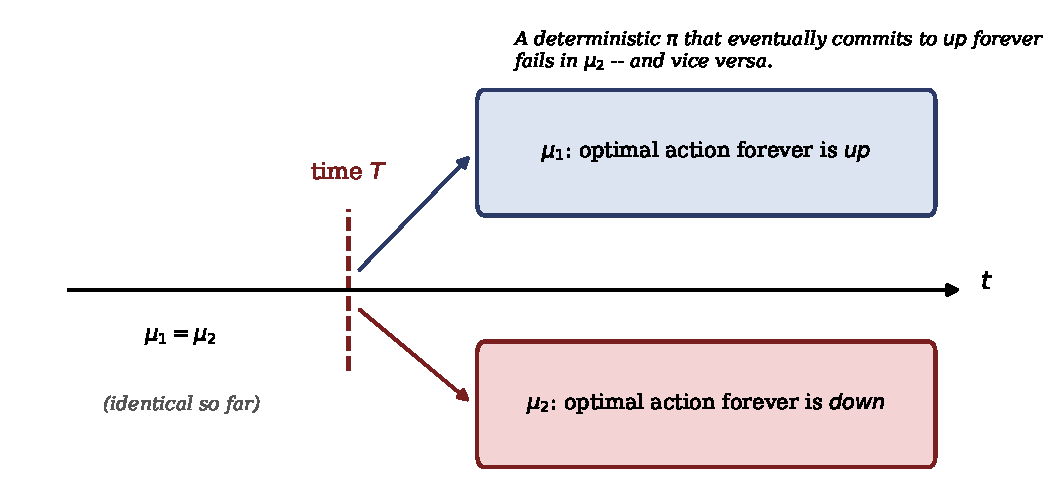
\includegraphics[width=0.62\textwidth]{adversarial_switch}
  \end{center}
\end{frame}

\begin{frame}{Theorem 8.3.2: No Weak Asymptotically Optimal Policy for General $\mathcal{M}$}
  Theorem 8.3.1 is a very general result -- since it includes all
  deterministic policies, it also rules out the Bayes-optimal policy AIXI.
  We can be even more general and show that there does not exist \emph{any}
  policy (not even a randomized one) achieving even the \emph{weakest}
  asymptotic-optimality notion, for the class of \emph{all} environments.

  \begin{block}{Theorem 8.3.2 (No weak asymptotically optimal policy for general $\mathcal{M}$)}
    If we consider $\mathcal{M}$ to be the class of \emph{all}
    environments, then there is no weakly asymptotically optimal policy
    for $\mathcal{M}$.
  \end{block}

  \textbf{Proof.} This comes from constructing an environment specifically
  \emph{tuned against} a given policy $\pi$ -- one where the reward for
  actions is chosen such that there will be the \emph{largest} difference
  between the value of actions taken by $\pi$ and the optimal actions.
  Since there are no restrictions on the computability level of the
  environments (unlike Theorem 8.3.1's $\Mcomp$), this construction is
  possible for \emph{any} policy $\pi$, computable or not. $\blacksquare$
\end{frame}

\begin{frame}[fragile]{Python: The Adversarial Time-$T$ Switch}
  A minimal simulation of the Theorem 8.3.1 construction: two environments
  agree up to time $T$, then require opposite actions forever.

\begin{lstlisting}[style=pythonstyle]
# correct action after T: "up" for mu1, "down" for mu2
correct = {"mu1": "up", "mu2": "down"}

# a deterministic policy eventually committing to a fixed action
committed_action = "up"

for mu, want in correct.items():
    v = 1.0 if committed_action == want else 0.0
    print(f"committed to '{committed_action}' -> value in {mu} = {v}")
\end{lstlisting}

  \textbf{Output.} value in \texttt{mu1} $=1.0$ (matches); value in
  \texttt{mu2} $=0.0$ (forever wrong). A deterministic policy that is
  strongly asymptotically optimal in $\mu_1$ must eventually commit to one
  fixed action, so it necessarily fails in $\mu_2$ -- Theorem 8.3.1's
  contradiction.
\end{frame}

\begin{frame}{Where Does This Leave Us?}
  The impossibility results above paint a bleak picture for the notion of
  asymptotic optimality for general history-based agents. But the
  situation is not as bad as it looks:
  \begin{itemize}
    \item The proofs crucially depend on the policy being
      \textbf{deterministic}. \textbf{Weak} (Theorem 9.4.1) and
      \textbf{strong} (Theorem 9.4.2) asymptotic optimality are actually
      \emph{achievable} by \textbf{stochastic} policies that add extra
      exploration to $\mathrm{AI}\xi$ (Section 9.4).
  \end{itemize}

  \bigskip
  \textbf{Open questions.} Which optimality criterion an artificial general
  intelligence would or should satisfy remains an open question:
  \begin{itemize}
    \item Should we conclude from the fact that $\mathrm{AI}\xi$ is
      \emph{not} strongly asymptotically optimal that we should use
      $\mathrm{Inq}$ (an exploratory variant), which \emph{is}?
    \item Or does $\mathrm{Inq}$ fare worse than $\mathrm{AI}\xi$ with
      respect to \emph{other}, possibly more important, optimality
      criteria?
    \item For instance, the \textbf{price} of asymptotic optimality is
      \emph{certain death} [CHC21] -- achieving it may require taking
      arbitrarily risky exploratory actions.
  \end{itemize}

  \bigskip
  Studying how these criteria relate to each other, and which are
  achievable under which conditions, helps narrow down desirable optimality
  criteria for both theoretical and practical artificial general
  intelligences.
\end{frame}

% =============================================================================
\section{8.4 Exercises}
% =============================================================================

\begin{frame}[allowframebreaks]{8.4 Exercises}
  \begin{enumerate}
    \item[1.] [C10] Prove that an agent is balanced Pareto optimal iff it is
      Bayes-optimal.
    \item[2.] [C20] Prove that strong asymptotic optimality implies both
      asymptotic optimality in mean and also weak asymptotic optimality.
    \item[3.] [C20] Give an example of an environment class $\mathcal{M}$
      and a family of policies $\{\pi_i\}$ such that no policy is Pareto
      optimal.
    \item[4.] [C20] Prove that geometric discounting satisfies Assumption
      8.1.11, and that all of the other discounting methods (power, finite
      lifetime, harmonic, hyperbolic, universal, no discount) from Table
      6.4 fail at least one of the three assumptions.
    \item[5.] [C15] Prove the equalities in (8.1.16).
    \item[6.] [C24] Prove that if $\mathcal{A}$, $\mathcal{E}$ are finite, a
      Pareto optimal policy exists.
    \item[7.] [C19] Prove that if $\pi$ is not Pareto optimal, then it is
      Pareto dominated by a Pareto optimal policy $\pi'$.
    \item[8.] [C24] Weaken the premises of Theorem 8.2.1 to no longer
      require that $V_\xi^\pi(h_{<t})>\varepsilon$. Prove that the action
      $\pi(h_{<t})$ is a $\xi'$-optimal action, but may not be uniquely
      optimal.
    \item[9.] [C15] Show that for all $\pi$, there exists an environment
      $\nu$ such that $\pi$ is not $\nu$-optimal.
    \item[10.] [C30] Formalize the proof of Theorem 8.3.1.
    \item[11.] [C18] Formalize the proof of Theorem 8.3.2.
    \item[12.] [C28] Provide a counter-example that convergence-in-mean does
      not imply Ces\`aro-convergence almost surely.
    \item[13.] [C20] Prove that convergence-in-mean implies Ces\`aro
      convergence-in-mean.
    \item[14.] [C23] Prove convergence almost surely implies Ces\`aro
      convergence almost surely.
    \item[15.] [C18] Provide a counter-example that weak asymptotic
      optimality does not imply asymptotic optimality in mean and a counter
      example that asymptotic optimality in mean does not imply weak
      asymptotic optimality.
    \item[16.] [C32] Derive an $\varepsilon$-optimal equivalent of the
      notions of optimality discussed in this chapter. How do they differ
      from the non $\varepsilon$-optimal versions? When are they
      equivalent?
  \end{enumerate}
  \explain{The bracketed numbers such as [C20] are the book's difficulty
    ratings for each exercise (roughly, ``C'' for a problem requiring
    creative/compositional reasoning, with the number indicating relative
    difficulty/length).}
\end{frame}

% =============================================================================
\section{8.5 History and References}
% =============================================================================

\begin{frame}[allowframebreaks]{8.5 History and References}
  \textbf{Notions of optimality.} This chapter is based on material from
  [LH15b] and [Lei16b, Chp.\,5]. Universal Bayesian agents were introduced
  in [Hut02c], which showed that $\mathrm{AI}\xi$ is
  \textbf{Self-Optimizing} and \textbf{Pareto-Optimal}. A comprehensive
  review of many of the notions of optimality discussed in this chapter and
  beyond can be found in [Hut05b, LH15b, Lei16b].

  \bigskip
  Related to regret and asymptotic optimality are the \textbf{PAC} and
  \textbf{sample-complexity} based optimality notions. Near-optimal PAC
  bounds for finite discounted MDPs based on Upper Confidence Reinforcement
  Learning (\textbf{UCRL}) [JOA10] have been proven in [LH12, LH14c]. The
  first PAC result in \emph{general} reinforcement learning was given in
  [LHS13b], with additional work being done in the case of feature
  abstractions being utilized in [RLDG22]. A simple but very general
  Bayesian regret bound covering and unifying many special cases was
  presented in [LVRD$^+$21].

  \framebreak

  \textbf{Asymptotic optimality.} The difficulty of asymptotic optimality
  was first demonstrated in [Ors10], where it was shown that AIXI is
  \emph{not} asymptotically optimal. These results were extended in
  [LH11a], where the authors defined two notions of asymptotic optimality
  and showed that under certain conditions these can(not) be satisfied. One
  of the difficulties with asymptotic optimality is that to achieve it, an
  agent needs to \textbf{explore} enough to gain sufficient information
  [RVR14, RCV16].

  \bigskip
  There are downsides to this exploration: in particular, it was shown that
  if an agent explores \emph{enough} to be asymptotically optimal, then it
  also explores enough to \textbf{die with certainty} [CHC21]. Algorithms
  able to achieve both asymptotic-optimality and regret-based optimality
  results, as well as the connection between the two, are presented in
  [KLVS21, LLOH16, Lei16b]. The existence of a policy able to achieve
  \textbf{strong} asymptotic optimality was proven in [CCH19].
\end{frame}

% =============================================================================
\begin{frame}{Summary}
  \begin{itemize}
    \item \textbf{$\nu$-optimality / $\varepsilon$-optimality}: the ideal
      but unrealistic gold standard -- optimal in one (possibly unknown)
      true environment.
    \item \textbf{Asymptotic optimality} (strong $\Rightarrow$ in mean, in
      probability $\Rightarrow$ weak): eventually optimal, in various
      probabilistic senses; connected to \textbf{sublinear regret} via
      Theorem 8.1.13 under recoverability.
    \item \textbf{Bayesian optimality}: optimal w.r.t.\ a mixture over an
      environment class; AIXI is Bayes-optimal in $\Msol$ with the
      universal prior; the ``best of both worlds'' criterion.
    \item \textbf{Regret minimization}: a finite-horizon, short-term
      notion, in tension with asymptotic optimality (Example 8.1.10).
    \item \textbf{Pareto optimality}: too weak alone (vacuous for
      $\mathcal{M}\supseteq\Mcomp$, Theorem 8.1.19), but its
      \textbf{balanced} refinement coincides exactly with Bayes-optimality.
    \item \textbf{Bad priors} (dogmatic, indifference) show that
      Bayes-optimality's behaviour \emph{depends heavily} on the prior --
      motivating the search for \emph{natural} universal priors.
    \item \textbf{Impossibility results} (Theorems 8.3.1, 8.3.2) show
      determinism and full generality are each obstacles to asymptotic
      optimality -- but stochastic exploration can restore it (Chapter 9).
  \end{itemize}
\end{frame}

\end{document}
